\documentclass[12pt]{article}

\usepackage{xcolor}
\usepackage{caption}
\usepackage{graphicx}
\usepackage{setspace}
\usepackage[margin=1in]{geometry}
\usepackage{hyperref}
\usepackage{cite}
\usepackage{placeins}
\usepackage{float}
\usepackage[utf8]{inputenc}
\usepackage[T1]{fontenc}
\usepackage{csquotes}
\usepackage{colortbl}
\usepackage{indentfirst}
\usepackage{makecell}
\definecolor{Gray}{gray}{0.85}
\newcolumntype{a}{>{\columncolor{Gray}}c}
\newcolumntype{b}{>{\columncolor{white}}c}

% align line-breaked column headers to the right
\renewcommand\theadalign{cr}

\begin{document}

% make section headers more reasonably sized, add italics
\makeatletter
\renewcommand\section{\@startsection {section}{1}{\z@}%
                                   {-1.5ex\@plus -1ex \@minus -.2ex}%
                                   {.75ex \@plus .2ex}%
                                   {\normalfont\normalsize\bfseries}}% 
\renewcommand\subsection{\@startsection{subsection}{2}{\z@}%
                                   {-1.0ex\@plus -1ex \@minus -.2ex}%
                                   {.5ex \@plus .2ex}%
                                   {\normalfont\normalsize\itshape}}%
\makeatother


\title{\vspace{-10pt} 
  Color-Blind Algorithmic Racism \\
  \large Race, Differential Privacy, and the 2020 U.S. Census}
       
\author{\vspace{-20pt} \normalsize \textit{Simon Couch\footnote{Thank you to Kaiyan Shi, Andrew Bray, and Adam Groce for their thoughtful insight on algorithmic considerations.}—11 May 2020}}

\date{}

\maketitle

%\doublespace

\vspace{-20pt}
\section{Introduction} \label{sec:intro}

\section{Background} \label{sec:background}


\subsection{The U.S. Census}\label{sec:census}

Article I, Section II of the U.S. Constitution mandated that an ``actual enumeration'' of the U.S. population should take place every ten years. The first census was taken in 1790, and since 1903, the Bureau has undertaken significant efforts not only to collect this data, but to distribute it in a useful and comprehensive manner. Resultantly, the Bureau now publishes billions of statistical summaries of this data following every decennial census for uses in legislative redistricting, distributing ``more than \$675 billion in federal funds,'' and social research, to name a few \cite{bureau_us_2020}.

The data is released at varying levels of detail: by nation, region, division, state, and county. The census also designates its own finer levels of observation: census tracts, block groups, and blocks. The census block group, which is the second smallest level of observation published by the Bureau and is increasingly a unit of analysis in social research, is the degree of detail centered in this paper: these areas can generally be imagined as, in a city, a literal group of city blocks, generally containing in the range of 900 to 1400 people (though possibly containing no people at all or tens of thousands) \cite{bureau_us_2020}.

\subsection{The Problem of Privacy}\label{sec:privacy}

The Bureau faces a dual mandate to publish summaries of the data they collect that are both accurate and protective of respondent privacy. These mandates are not just customary, but enshrined in law \cite{code_title_1954, code_title_2002}. The strategies employed by the census to protect respondent privacy in practice are referred to as `disclosure avoidance processes.'

In past censuses, disclosure avoidance was largely an ad-hoc procedure carried out at the discretion of Bureau analysts, consisting of `swapping' households from one block to another or adding small amounts of mathematical randomness to population counts. These procedures were critically important for respondents who might be, for example, the only whom identified with some racial category in a census block. As a result, analysts who wished to uncover information about specific respondents would be unable to discern whether some entry in published statistics truly represented the presence of a known respondent or was the result of the swapping of households or addition of noise. In the past, the guidelines for carrying out these procedures, as well as clarification on which data products are impacted by this process, remained internal to the Bureau \cite{boyd_balancing_2020}.

Recently, however, it has become clear that improvised or arbitrarily determined privatization techniques are not sufficient to protect respondent privacy. The swaths of data that the census publishes, as with any data, are vulnerable to database reconstruction attacks, whereby some attacker attempts to reconstruct the `original' data from its summaries by combining the data with other data summaries as well as third-party data sources. (Third-party data sources might include state records or personal data collected from smartphones.) More data available for attackers to combine with census data means a greater probability that attackers will be able to transform statistical summaries into individual records. In other words, it is possible that, with enough detailed data on a sensitive population, one may be able to reverse engineer the underlying data used to generate the summaries, and thus reveal sensitive information about individual respondents. Taken in conjunction, the massive increase in computing power available to individuals and data on people hosted throughout the internet means that the results of the Census are increasingly vulnerable to reconstruction attacks \cite{boyd_balancing_2020, abowd_economic_2019}. In realization of this risk, the Bureau announced in 2018 that it would be taking further steps to protect respondent privacy.

\subsection{Differential Privacy}\label{sec:dp}

Differential privacy is an emerging field at the intersection of statistics and computer science. Differentially private algorithms seek to optimize the statistical utility of (in this case) data summarizations while also mathematically provably protecting the privacy of individuals. They do so by guaranteeing that statistical summaries will not change `too much' depending on whether a specific individual is in the dataset or not, where the notion of `too much' is parameterized by an epsilon $\epsilon$ value sometimes referred to as a `privacy-loss budget.' To carry this out, algorithms add small amounts of noise to the true outputted statistics in order to produce public data summaries. Thus, the consumer of the differentially private estimates cannot be certain whether the relationships in a set of summary values are due to the presence of a specific individual in the database, or are simply the result of the addition of random noise. As a result, though, there is inherently a trade-off between confidentiality and statistical utility.

The Bureau's choice of differentially private algorithms offers several unique advantages over the previous approach:

\begin{itemize}
  \item \textit{Robust to post-processing}: Differentially private algorithms are robust to post-processing, meaning that the privacy guarantee of an algorithm is not comprimised by processing (e.g. rounding population counts to the nearest whole number or rounding negative population counts up to zero) the outputted data as long as the original, true values are not accessed as part of the computation. This also means that the Bureau can adjust for what it terms \textit{invariants}, which are certain selected values whose true value must remain unaltered. For example, the Bureau could scale privatized county population counts to ensure that they add up to the total state population.
  \item \textit{Public}: Unlike the Bureau's previous approach, all details of the implementation of the differentially private algorithm can be made available without comprimising the privacy guarantee. This will allow for analyses based on the released data to statistically account for the addition of noise. This also means that the code used to implement the Bureau's algorithm can be publicly vetted for accuracy and rigor.
  \item \textit{Straightforward Composition}: When a statistic is derived from combining the output of an $\epsilon_1$-differentially private algorithm and an $\epsilon_2$-differentially private algorithm, that statistic is at most $\epsilon_1 + \epsilon_2$-differentially private. This means that the Bureau can release as many $\epsilon_i$-differentially private summaries as necessary, and can straightforwardly guarantee that the complete data product is ($\sum_i \epsilon_i$)-differentially private.
\end{itemize}

Since the Bureau's announcement of this decision, there has been considerable resistance from a variety of stakeholders---for many, ``the idea that data utility and privacy can be operationalized into a mathematical trade-off is both unfathomable and deeply unsettling'' \cite{boyd_balancing_2020}. In Section \ref{sec:results}, I will argue that this wariness is well-founded.

% Those who have been deeply invested in understanding the details of the census know that disclosure avoidance mechanisms have always introduced some noise into the system, but the bureau has always maintained that the noise purposefully introduced is very small compared to the noise that comes from mistakes, imputation, and other forms of human error. Data users have accepted – or, in some cases, not known about – this reality. \cite{boyd_balancing_2020}

\subsection{Census Racial Categories}\label{sec:race-cats}

In the social sciences, it is well-accepted that race and ethnicity are socially constructed categorizations. Considerable work has been devoted to examining exactly what it means for such socially salient concepts to be social constructions \cite{lee2009race, omi_racial_2014}, largely converging in their consensus that historical theorizing on race ``has been part and parcel of rac\textit{ism}'' \cite{morning2011nature}. ``Since its invention to manage the expansion of European enslavement and the colonization of other peoples, the definitions, criteria, and boundary lines that determine racial categories have constantly shifted over the course of U.S. history'' \cite{roberts2011fatal}. The decennial census is a unique window into this history, exemplifying the instability and arbitrariness of racial categorizations. 

Every decade since the first census in 1790, the Bureau has somehow altered the `race question,' whether it be in its phrasing, the categories offered, or instructions on choosing them \cite{strmic-pawl_race_2018}. Many have written on this history \cite{espiritu_asian_1992, prewitt_what_2013, strmic-pawl_race_2018, hochschild_racial_2008}, and conclusions are shared among many theorists: ``For the majority of the existence of the census, Whiteness and power motivated the addition and removal of racial groups, the names for racial groups, and the use of census officials to observe and record the race of participants,'' and, consequently, ``the categories have been arbitrary and inconsistent---often reflecting the Census Bureau’s administrative needs rather than the population's perceptions of meaningful cultural and racial differentiations'' \cite{espiritu_asian_1992, strmic-pawl_race_2018}. Pre-civil rights era, the inclusion of racial categorizations in the census was largely a tool for subordination, but after the 1960s, the bureau adopted a ``social equity ideology'' \cite{strmic-pawl_race_2018}. The latter half of the 20th century, especially, saw significant variation in the construction of Asian and Hispanic categorizations, and the terminology used to refer to them (whether racial, ethnic, ethno-racial, or the more self-aware ``super-ethnic'') \cite{espiritu_asian_1992, choldin_statistics_1986}. This reorientation is not simply a reflection of organizational conscience; the U.S. Commission on Civil Rights ``stated that racial and ethnic classification can be justified only if the data produced have a legitimate use in terms of combating discrimination, planning programs, or conducting program evaluation'' \cite{humes_measurement_2009}. We can thus see that the Bureau’s choice of racial categorizations is situationally determined--I also argue that this choice is highly consequential.

\subsection{``Race Counts''}\label{sec:race-counts}

Not only is accurate census count mandated in Article I, section II of the U.S. Constitution, but it is an absolute necessity for the functioning of democracy. Accurate census counts by race bear on the electoral process, claims of discrimination, the distribution of money to local governments and grant applicants, and research in a plethora of fields. 

For one, population statistics are used to ensure fairness in accessibility to the electoral process. The 1975 Voting Rights Act requires that ``bilingual assistance must be available in voting districts in which more than 5 percent of the citizens are members of the affected language minority group'' \cite{espiritu_asian_1992}. Counts by race, then, were especially important in planning for the 1980 census, where, because the 1970 census did not ask about languages spoken in the home, racial statistics were used as a proxy for language accessibility needs \cite{keane_increasing_1985}. Since then, too, if one grants that non-English-speaking needs are not equally distributed among census racial categories, an inaccurate count by race implies an inaccurate understanding of language accessibility needs. Not to mention, too, that beyond language accessibility needs, census counts directly determine the apportionment of seats in Congress.

Additionally, underrepresentation is the basis of many affirmative action cases, and proportions by race based on census enumeration have successfully been used as evidence in such cases \cite{harris_whiteness_2003, espiritu_asian_1992, choldin_statistics_1986}.

Further, population counts ``bear directly on the distribution of federal monies to states, counties, and cities for everything from feeding the poor to running mass transit systems.''  Similarly, billions of dollars a year in grant money are distributed at least in part according to census counts, especially those figures that are tied to economic and health disparities \cite{espiritu_asian_1992}.

% in coming together to lobby for more thoughtful and comprehensive representation in the 1990 U.S. census, Asian Americans ``did not merely accept the pan-Asian concept imposed by outsiders but also used it to advance their political demands—including the demand that government bureaucracies treat them as separate groups within a larger category.'' \cite{espiritu_asian_1992}

% ``Local public officials also entered into the undercount controversy. Besides affecting the apportionment of seats in Congress, seats in state legislatures, and even city council distncts, census population counts bear directly on the distribution of federal monies to states, counties, and cities for everything from feeding the poor to running mass transit systems.'' \cite{maurice_census_1982}

\subsection{A Note: Defining Race}\label{sec:defining-race}

In this paper, my use of the term `race' will largely mirror that of Prewitt's \textit{statistical race}: ``Organized counting of any kind---and certainly a census is organized counting---requires counters to know what they are counting, which in turn depends on a classification scheme. Statistical races are by-products of the categories used in the government’s racial classification.'' \cite{prewitt_what_2013} The statistical races (and ethnicities) referenced in this paper, then, are those that result from the 2010 and 2020 census racial classifications. It is worth noting that the census' use of the term race refers to an undifferentiated conglomeration of definitions and concepts invoking biological race \cite{prewitt_what_2013, quisumbing_king_recentering_2019}, ethnicity and panethnicity \cite{omi_racial_2014, espiritu_asian_1992, espiritu_who_2000}, nationality \cite{mezey_erasure_2002}, and existing sovereign nationhood \cite{byrd_been_2011}. Further, consistent with the Bureau's current analytical approach \cite{pack_note_1996, fox_differential_2018}, I will consider respondents who identify as non-Hispanic/Latino ethnically and white racially as white people, and those who do not as people of color, as binary analytical categories in some analyses in Section \ref{sec:results}. The relationship between statistical races and whatever phenomenon they proxy is left to Section \ref{sec:disc}.
  

\subsection{The Differential Undercount}

Some of the census statistics use cases in Section \ref{sec:race-counts} may not seem, at the surface, inherently racialized. This is not the case, though, given the existence of ``differential undercounts,'' where the counts of certain population segments are systematically lower than their actual count to a greater proportion than other segments. That is, the severity with which population groups are not sufficiently counted is not evenly distributed amongst age groups, geographic areas, gender identities, races, ethnicities, and tribal statuses. Notably, ``the undercount rate for racial and ethnic minority groups is substantially higher than the undercount rate for other demographic criteria'' \cite{fox_differential_2018}. Indeed, ``[t]he 1990 census also missed more minorities than whites, undercounting about 5 percent of blacks and Latinos while overlooking fewer than 2 percent of whites'' \cite{espiritu_asian_1992}. Given this fact, and the continuing severity of geographic segregation in the U.S. \cite{bonilla-silva_racism_2010}, \textit{any} count inaccuracy is inherently racialized. 

There are several sources contributing to a racialized differential undercount. Principally, recent literature has pointed to the well-founded fears of minorities in disclosing membership in marginalized groups. Distrust of the Bureau, and the U.S. government in general, is often argued to contribute significantly to the differential undercount, especially in reference to (recently) historical disclosures of constitutionally protected confidential information on the part of the Bureau to other divisions in the Executive Branch. Especially in light of recent violences perpetrated by the Trump administration, as well as the debate on the addition of a citizenship question to the 2020 Census, scholars predict that ``Hispanic distrust of the government will lead to an unprecedented differential undercount in the 2020 Census'' \cite{fox_differential_2018}. See Section \ref{sec:disc} for more discussion of Bureau disclosures of constitutionally protected information and enabling of government-perpetrated violences.

\subsection{Color-Blind Racism}\label{sec:color-blind}

In his oft-cited book \textit{Racism Without Racists}, Eduardo Bonilla-Silva describes the ideology of \textit{color-blind racism}, referring to the dominant and powerfully dismissive American racial ideology that ``explains contemporary racial inequality as the outcome of nonracial dynamics'' \cite{bonilla-silva_racism_2010}. Assuming the absence of institutionalized racism and refusing to reconcile persistent racialized inequality beyond blaming ``imputed cultural limitations,'' this framing holds to the abstractly liberal ideas of universalism and equality, claiming that color-blind efforts to address economic inequality will benefit all equally. As Justice Roberts famously wrote in his plurarity opinion on Parents Involved in Community Schools v. Seattle School District No. 1, this ideology would agree that ``[t]he way to stop discrimination on the basis of race is to stop discriminating on the basis of race.'' 

The Bureau's implementation of differentially private algorithms to estimate the results of the 2020 U.S. Census is a glaring example of color-blind racism. These algorithms will be used to estimate the population counts of people in the U.S. by race and ethnicity in a color-blind manner, meaning that the same amount of mathematical randomness will be added to all racial and ethnic subgroup counts. Given the racial taxonomy used by the Bureau, though, on average, there will be significantly fewer people identifying with a given ethnoracial subgroup other than White non-Hispanic/Latino than there will be those who identify with the White non-Hispanic/Latino subgroup. As a result, since the same amount of noise is added to each subgroup count, the estimates for subpopulations of people of color will be significantly worse than those for white people.

A simulation of this phenomenon is shown in Figure \ref{fig:dif-priv}. This figure supposes two hypothetical populations, A and B, for which the true population counts are 50 and 1000, respectively. Supposing that the populations were counted correctly, the counts are processed using a `differentially-private' algorithm, where the same amount of noise is added to both population counts. However, this noise is much more meaningful for population A, with estimated population counts sometimes dipping into the negatives, and often being half or twice the actual population size. This same error distribution for population B, however, by proportion, is much less meaningful; underestimating a population count of 50 by 50 is a much more drastic change than underestimating a population count of 1000 by 50. If these population counts were counts by race, then, the issue of a color-blind algorithm (and, possibly, the use of this class of algorithm in general) becomes clear. 

\begin{figure}[ht]
   \centering
   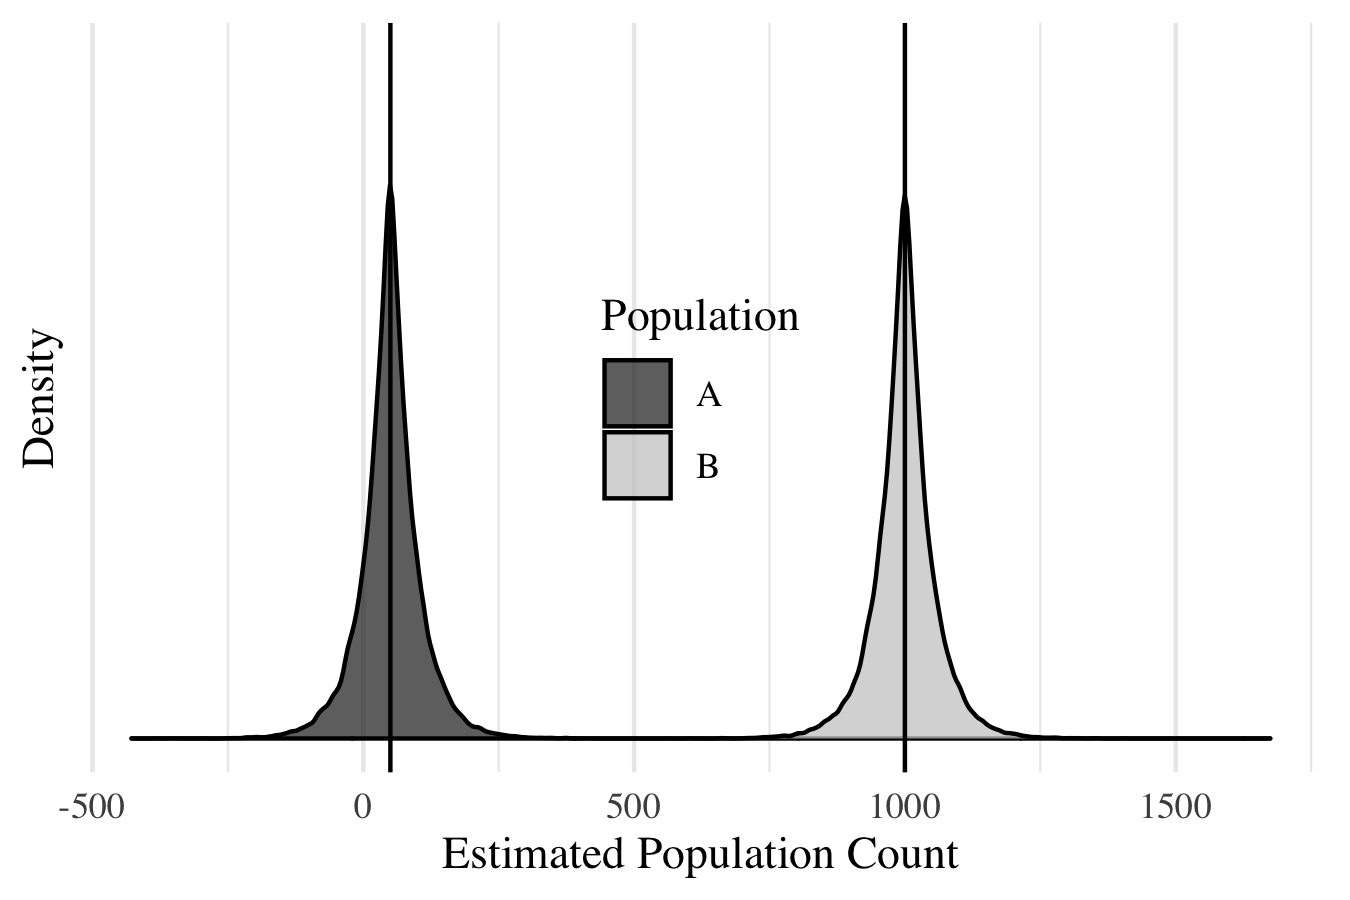
\includegraphics[width=0.75\textwidth]{figures/dif_priv.png}
   \caption{Distributions of `differentially private' population count estimates for hypothetical populations A and B, with respective true population counts of 50 and 1000. The variance of the error in each distribution is identical, but is much more meaningful for the accuracy of the estimate for population A than for B.}
   \label{fig:dif-priv}
\end{figure}

How does this hypothetical scenario play out in practice, though? I will show in Section \ref{sec:results} that the implementation of this privatization algorithm for use in the 2020 U.S. Census is a particularly egregious example of color-blind racism in action. This decision by the Bureau will disproportionately negatively impact people of color, and, further, if Fox \cite{fox_differential_2018} was correct in arguing that the differential undercount already likely in the 2020 U.S. Census undermines Article I, Section II of the U.S. Constitution, then so too is the implementation of differentially private algorithms for use in privatizing the results of the 2020 U.S. Census.

% Let not the irony be lost of the census choosing a class of privatization algorithms called ``differentially private'' that will aggravate the differential undercount problem.


\section{Data \& Methods}\label{sec:methods}

The data used in this paper is a subset of data released by the Bureau in early 2019 consisting of the output from a trial run of the differentially private algorithms on the publicly available 2010 Census data product \cite{bureau_2010_2019}. To facilitate more straightforward comparison, the Integrated Public Use Microdata Series National Historical Geographic Information System (IPUMS NHGIS) released a set of datasets containing the `true' (though privatized with the procedures described in Section \ref{sec:privacy}) data joined to the files containing the differentially private estimates \cite{manson_differentially_2019}. The data files analyzed in this project come from the Block Group (150) level, wide format file.

The analyses in this paper are limited to basic visualizations and tabulations of the original data. The focus of the analyses is the quality of estimation by race and ethnic categories at the census block group level. The choice of metrics of estimation quality are largely arbitrary, chosen to communicate estimation (in)accuracy in the most interpretable way possible. Throughout the analysis, I often refer to `percent error' of an estimate. If $x_{T}$ is some true summary value (subject to the privatization techniques described in Section \ref{sec:privacy}), and $x_{P}$ is the differentially private estimate of the summary value, then the percent error is given by $$(x_P - x_T) / x_T * 100$$ Thus, a percent error of 0\% means that the differentially private estimate was exactly equal to the true value, a percent error of 100\% means that the differentially private estimate was twice as large as the true value, and a percent error of $-100$\% means that the differentially private estimate was zero, while the true value was nonzero. As part of the Bureau's post-processing, negative estimates are rounded up to zero---thus, the minimum percent error in the data is $-100$\%. The maximum percent error is not bounded.

Fully reproducible scripts for downloading, transforming, tidying, visualizing, and analyzing the data are publicly available\footnote{Source code publicly available at: \url{https://github.com/simonpcouch/dp_census}}. 









\section{Results}\label{sec:results}


Figure \ref{fig:error-true-pop} examines how the hypothetical distributions proposed in Figure \ref{fig:dif-priv} appear in practice. The upper pane gives the distribution of population counts by racial category---the typical population counts within a census block group for people of color are significantly lower than those for white people. The lower pane, then, shows how a color-blind algorithm can have such a racialized effect. While the algorithms are not sensitive to whether they are estimating population counts for people of color or white people, they perform much worse (in that the absolute magnitude of percent error is much greater) when estimating smaller population counts, which are much more likely to belong to populations of color than to white populations.

\begin{figure}
   \centering
   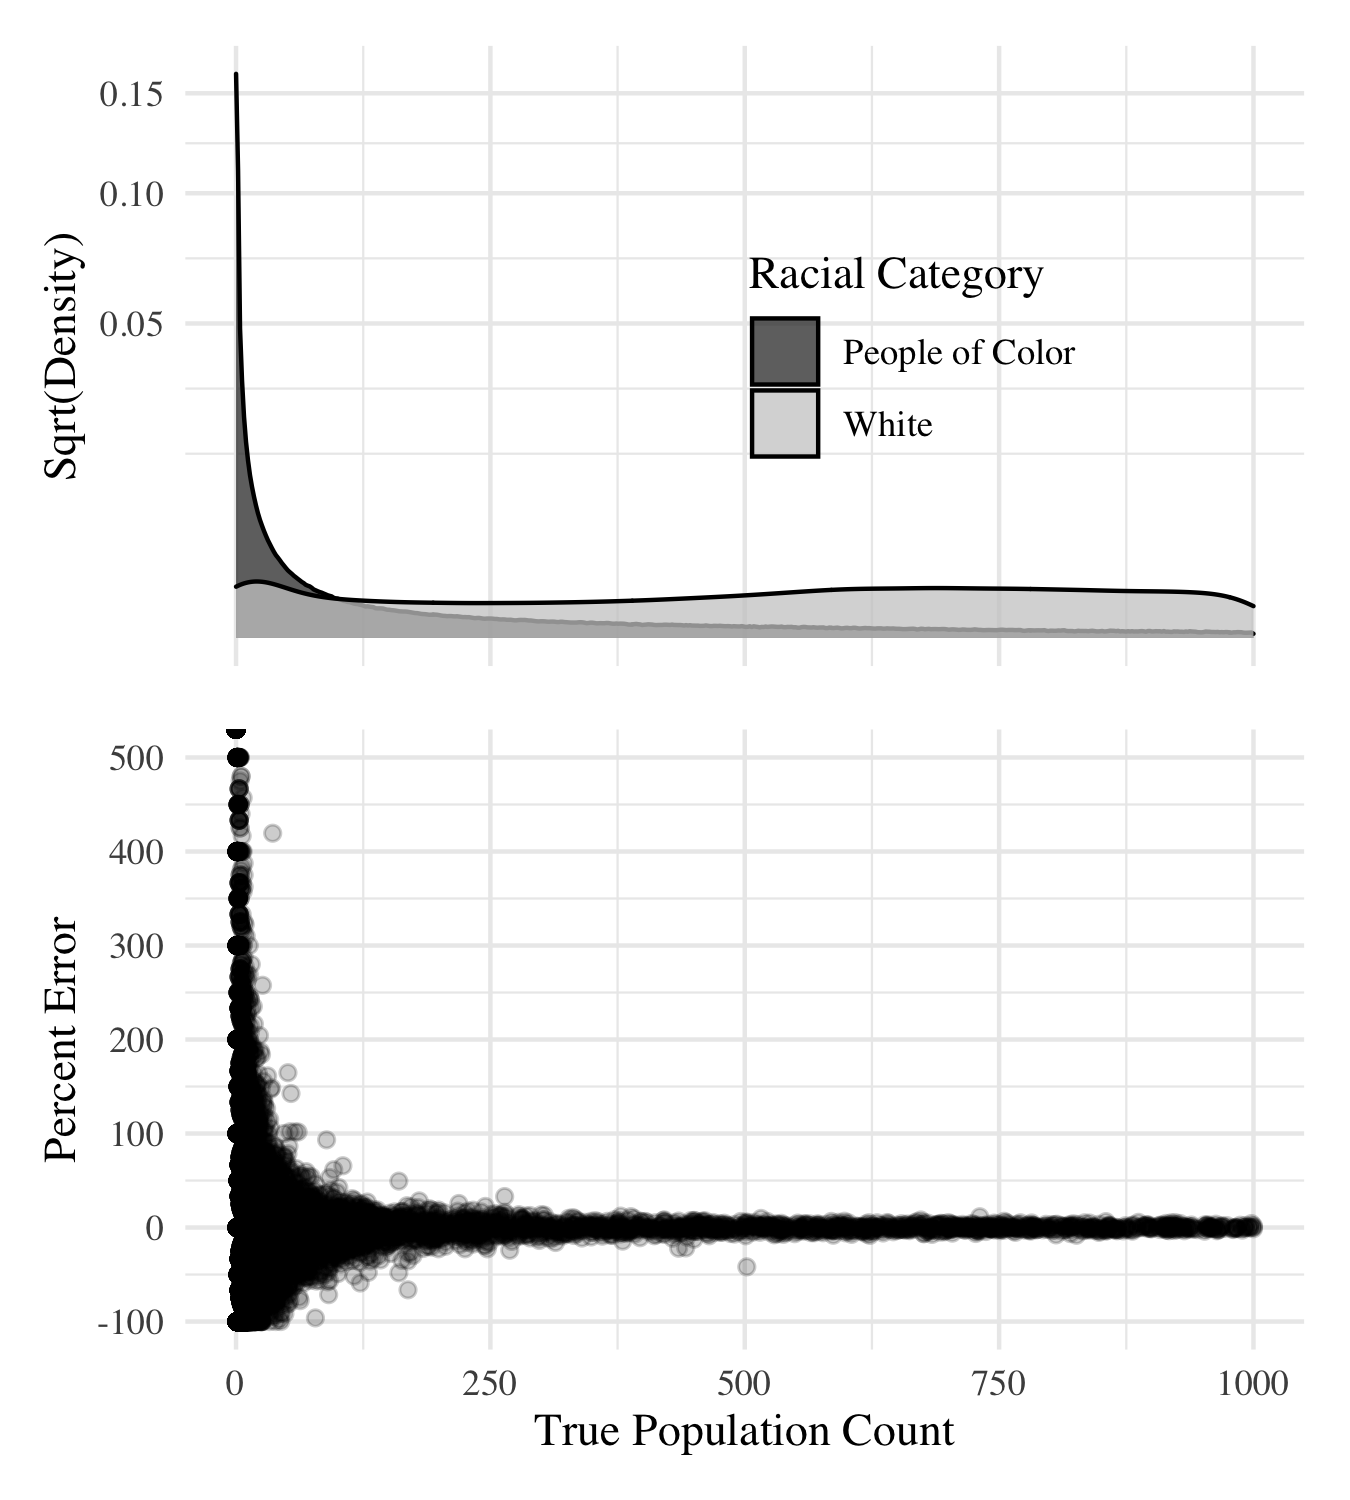
\includegraphics[width=0.75\textwidth]{figures/error_by_true_pop.png}
   \caption{A pair of plots showing the distribution of true population counts by census block group from the 2010 U.S. census, where the upper pane delineates the density by racial category, and the lower shows the distribution of percent error between true population count and differentially private estimate. Lower population counts are both more likely to occur when describing populations of color and more susceptible to significant error in estimation.}
   \label{fig:error-true-pop}
\end{figure}

Figure \ref{fig:error-by-race}, then, shows the implications of implementing differentially private algorithms in a use case such as that shown in Figure \ref{fig:error-true-pop}. In the trial run on 2010 Census data, the distributions of percent error have substantially greater variances for populations of color than for white populations. Further, too, the only distribution of percent error centered around zero is that of white populations; roughly in accordance with the absolute population size, the distribution of percent error is centered closer and closer to $-100$\% (complete erasure.) The Native Hawaiian and Pacific Islander categorization shows a particularly egregious example of this effect, with over 50\% of nonzero population counts completely erased. The fact that some of these distributions are centered around nonzero numbers should be puzzling to those familiar with differentially private algorithms, and is likely a result of post-processing and adjusting for invariants carried out by the Bureau.

\begin{figure}
   \centering
   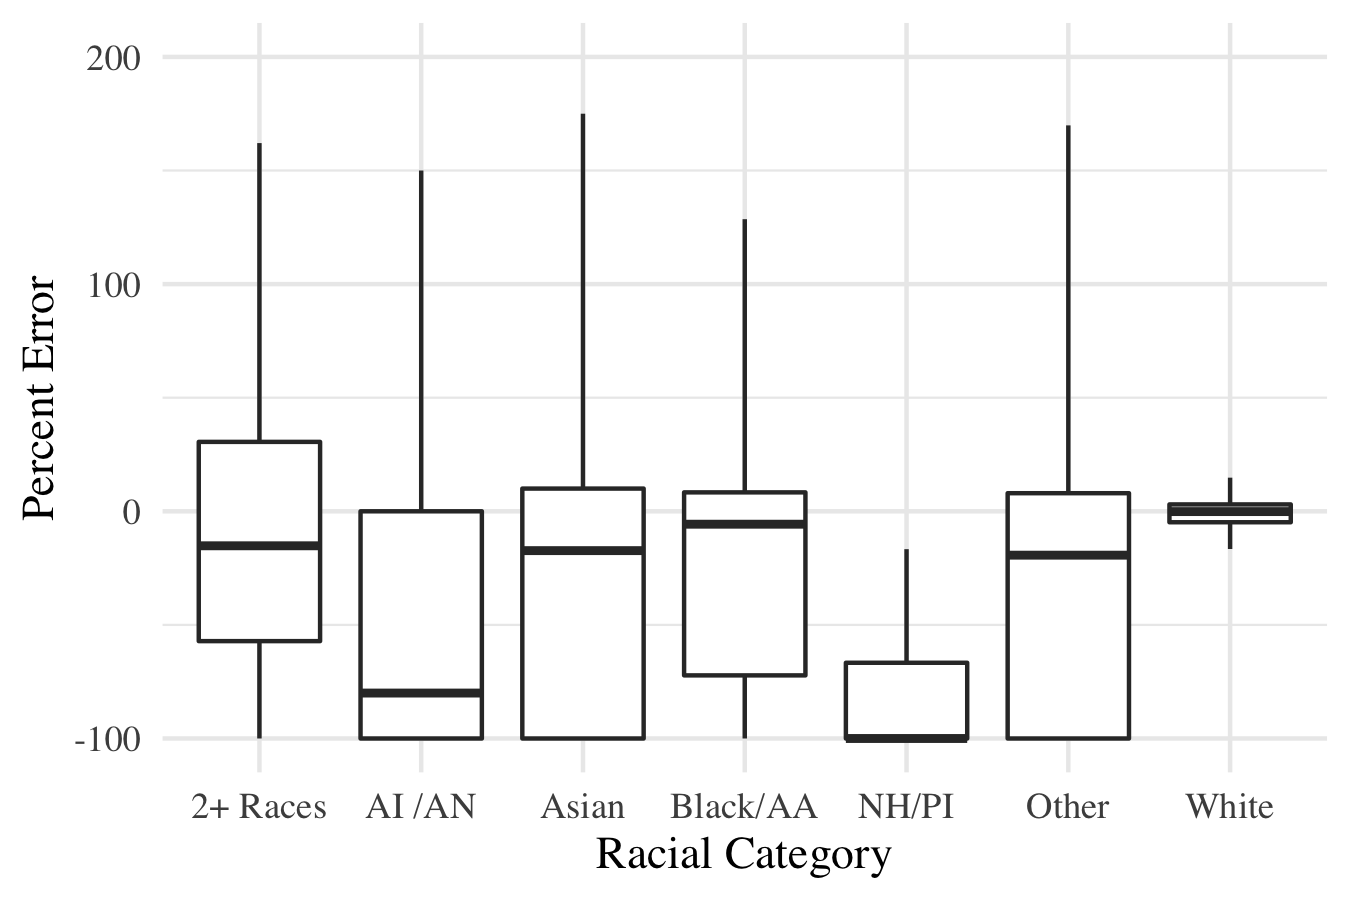
\includegraphics[width=0.75\textwidth]{figures/error_by_race.png}
   \caption{Distributions of percent error in estimation of true census block group population count by racial category. White populations experience, by far, the least deviation between true and estimated population counts, as well as the only distribution of percent error centered around zero.}
   \label{fig:error-by-race}
\end{figure}
 
\subsection{Erasing Races}\label{sec:erase}

Table \ref{tab:error-by} gives the proportion of estimates, by ethnoracial group, that experience abitrarily selected severities of error. Initially, consider the \textit{Population Erased} column, giving the proportion of nonzero populations estimated to contain zero people. For one, more generally, the proportion of populations erased by these algorithms is much greater for racial groups that identify as Hispanic/Latino than for those who do not. As before, smaller populations are increasingly subsceptible to this error; populations of people categorized as Hispanic/Latino Native Hawaiians or Pacific Islanders are erased in over 84\% of trials, and \textit{half} of the ethnoracial population subgroups are erased in at least 37\% of trials. By contrast, white populations are erased in less than 1\% of trials.

Similar disparities in estimation accuracy occur in the remaining three columns. While populations of color are also more likely to have their population counts drastically \textit{over}estimated, I contend that this is not cause for relief. The noise added to a statistic in the privatization process is completely independent of trial. That is, the previous perturbation of a population's true count has no bearing on the next. Resultantly, this overestimation is likely a `one-time' occurence, and, by the appearance of the distributions shown in Table \ref{tab:error-by}, is particularly vulnerable to complete erasure in the next census. As a result, drastic overestimation is also not an acceptable form of error, as it is simply an indicator of  instability.

% latex table generated in R 3.6.3 by xtable 1.8-4 package
% Mon May  4 10:50:06 2020
\begin{table}[ht]
\centering
\begin{tabular}{l|rrrr} 
 Ethnicity/Race Category & \multicolumn{4}{c}{Proportion of Estimates Resulting in Given Degree of Error} \\
 \hline
 & \thead{Population \\ Erased} & \thead{Less Than Half of \\ the True Population} & \thead{Twice the True \\ Population} & \thead{Ten Times the \\ True Population} \\ 
  \hline
H/L: 2+ Races & 0.179 & 0.179 & 0.107 & 0.014 \\ 
H/L: AI /AN & 0.469 & 0.469 & 0.087 & 0.009 \\ 
  H/L: Asian & 0.663 & 0.663 & 0.069 & 0.007 \\ 
  H/L: Black/AA & 0.379 & 0.379 & 0.088 & 0.009 \\ 
  H/L: NH/PI & 0.841 & 0.841 & 0.033 & 0.004 \\ 
  H/L: Other & 0.115 & 0.115 & 0.061 & 0.007 \\ 
  H/L: White & 0.055 & 0.055 & 0.029 & 0.002 \\ 
   \hline
Non-H/L: 2+ Races & 0.044 & 0.044 & 0.064 & 0.006 \\ 
  Non-H/L: AI /AN & 0.407 & 0.407 & 0.095 & 0.009 \\ 
  Non-H/L: Asian & 0.132 & 0.132 & 0.068 & 0.007 \\ 
  Non-H/L: Black/AA & 0.089 & 0.089 & 0.041 & 0.004 \\ 
  Non-H/L: NH/PI & 0.612 & 0.612 & 0.072 & 0.007 \\ 
  Non-H/L: Other & 0.529 & 0.529 & 0.094 & 0.009 \\ 
  Non-H/L: White & 0.006 & 0.006 & 0.005 & 0.000 \\ 
  \end{tabular}
  \caption{Proportion of estimates, by census ethnicity/race category, that result in selected degrees of estimation error. White, non-Hispanic/Latino populations are consistently well over an order of magnitude less likely to have their population erased by the differentially private algorithm than other ethnoracial categories. In general, the variability in differentially private population count estimates for populations of color is significantly greater than that for white populations.}
  \label{tab:error-by}
\end{table}

\subsection{Creating Races}\label{sec:create}

Another possible outcome resulting from the implementation of these algorithms is the estimation of positive subpopulation counts for subpopulations that do not exist. Table \ref{tab:nonzero-by} gives the proportion of cases in which this form of error occurs by ethnoracial category. Similarly to Table \ref{tab:error-by}, subpopulations are increasingly vulnerable to this form of inaccuracy as the true subpopulation size decreases.

% latex table generated in R 3.6.3 by xtable 1.8-4 package
% Mon May  4 10:50:08 2020
\begin{table}[ht]
\centering
\begin{tabular}{l|r}
 Ethnicity/Race Category & \thead{\% Estimated \\ Nonzero Count} \\ 
  \hline
  H/L: 2+ Races & 0.081 \\ 
  H/L: AI /AN & 0.171 \\ 
  H/L: Asian & 0.212 \\ 
  H/L: Black/AA & 0.135 \\ 
  H/L: NH/PI & 0.337 \\ 
  H/L: Other & 0.039 \\ 
  H/L: White & 0.012 \\ 
   \hline
  Non-H/L: 2+ Races & 0.009 \\ 
  Non-H/L: AI /AN & 0.064 \\ 
  Non-H/L: Asian & 0.042 \\ 
  Non-H/L: Black/AA & 0.018 \\ 
  Non-H/L: NH/PI & 0.206 \\ 
  Non-H/L: Other & 0.149 \\ 
  Non-H/L: White & 0.001 \\ 
  \end{tabular}
  \caption{Proportion of nonexistent populations that were estimated to have some nonzero population count by the differentially private estimators. White, non-hispanic/latino populations are at least an order of magnitude less likely to experience this misestimation than those in other ethnoracial categories.}
  \label{tab:nonzero-by}
\end{table}

















\section{Discussion}\label{sec:disc}

In the preceding section, I showed that the quality of differentially private population count estimates for populations of color at the census block group level is unacceptable at best. This result leaves much to be said to make meaning of these inaccuracies and consider possible remedies. My considerations of these problems omit the possibility of the most obvious solution: better algorithms. As many working on these problems have noted, however, the time to wait for technical innovation is not a luxury that is available to the Bureau.

Before the announcement that the Bureau would be using differentially private algorithms to privatize their data products, significant research was already being carried out making meaning of the racialized differential undercount. Specifically, several authors centered the question of how to structure ``the race question'' to most effectively inform social justice efforts within practical constraints.

One consideration coming out of this literature is to more closely examine the relationship between contempary understandings of racialized identity and the form of `the race question.' Does the Census' race definition need to reflect ``the population's perceptions of meaningful cultural and racial differentiations'' in order to most effectively serve its supposed new purpose of advancing social equity \cite{espiritu_asian_1992}? For one, census racial categorizations ought to be sensitive to previous (mis)uses of census racial data as well as the current political climate. In light of recent violences perpetrated by ICE and the Trump administration on Latinx people \cite{fox_differential_2018}, and the Bureau's role in surveillance of Arab Americans post-9/11 \cite{beydoun_demographic_2015}, Japanese American internment \cite{anderson_public_2015}, and displacement of Native Americans, ``all minorities share equally in the fear of answering race, ethnicity, and citizenship questions on the census'' \cite{fox_differential_2018}. If the ultimate end of the development and maintenance of census racial categories is the effective tracking of social inequality, and the identification with some specific racial and ethnic groups exacerbates an already severe differential undercount of racial and ethnic minorities, then the most effective categorizations might not necessarily reflect lived contemporary racial identity. As Fox wrote in a recent article on the differential undercount, ``[i]f you are in some other category a decade later, and millions are, you have changed your mind. Racial identity in the census is not whether a taxi stops for you, or what is on your birth certificate, or what your grandparents thought they were. It is a tick in a box.'' \cite{fox_differential_2018}

Further, too, what is a privacy promise worth when the Bureau systematically violates this promise? As mentioned earlier, the Bureau has violated its confidentiality promise by distributing census data throughout executive branch departments on multiple occasions. (See \cite{fox_differential_2018} for an exhaustive list of examples.) Historically, the Bureau has shown that it is incapable of truthfully promising confidentiality to constituents. Why, then, feign a struggle to reconcile privacy and statistical utility when the former is simply not a promise that the Bureau can make? In this way, the effect of the implementation of a `privacy-protection' algorithm---especially one that disproportionately harms people of color---seems futile at best, and gravely harmful at worst. Given that the Bureau has consistently failed to follow through on its commitment to respondent privacy, the census ought to reflect information that the constituency is comfortable being made public, and the Bureau should focus on ensuring that this data is as accurate as possible to fulfill its obligation to Article I, Section 2 of the constitution. Otherwise, significant efforts need to be undertaken to ensure respondent privacy beyond the narrow realm of reconstruction attacks and address the increasing risk of an unprecedented differential undercount. ``With this understanding of history and likely future practice, only a constitutional amendment barring government census disclosures will ensure that all residents may comfortably participate in the U.S. Census'' \cite{fox_differential_2018}. Otherwise, we must reckon with unrepresentativeness that will ``weaken policy choices relevant to economic growth, social justice, immigrant assimilation, government reforms, and an enlightened public'' \cite{prewitt_census_2018}.

Another possibility is the reconsideration of the geographic precision at which to release these statistics. Though data at the census block level is desired by many stakeholders, this level of detail is increasingly a risk to respondent confidentiality. As a result, too, the portion of the $\epsilon$ budget alloted to estimating block-level statistics could be reallocated to estimating other statistics, thereby increasing the quality of the published data \cite{boyd_balancing_2020}.

This study is limited in several key ways. Notably, for one, I only analyzed simulation data at the census block group level. With Figure \ref{fig:dif-priv} in mind, the results from the block group level are a (second-to) worst-case evaluation of the effects of the implementation of these algorithms. As population counts grow larger, the effect of privatization on the utility of these numbers will decrease. A more detailed study would examine each level of geographical organization, examining the effects of privatization at each level and discussing the implications for use cases of data especially relevant to that level of aggregation. Further, this paper makes use of the output of an existing algorithmic implementation. Further work would more closely consider the effect of varying parameterizations through the simulation of original datasets with many different choices of the total $\epsilon$ privacy budget and allocation of $\epsilon$ to different statistics, as well as run several iterations of the simulations in order to allow for more detailed study of the variation of the statistics describing specific geographic regions.

Altogether, I have argued that the implementation of differentially private algorithms to estimate subpopulation counts in the 2020 U.S. will have a disproportionately negative impact on the quality of count estimates of populations of color. This effect will exacerbate the existing differential undercount problem, where the Bureau systematically undercounts populations of color more so than it does for white populations.





\clearpage

\bibliographystyle{plain}
\bibliography{sources.bib}

\clearpage

%\appendix
%\section{Appendix}\label{sec:appendix}

\end{document}
